\chapter{System Evaluation}
This chapter evaluates the project against the objective set out in the introduction. Results are presented, discussing the system's strengths and weaknesses, and providing key insights into it's overall performance and effectiveness. The process is discussed to evaluate ConnectSphere as a social media platform.

\section{Project Planning}
The project was managed by Jira to help organize tasks and track progress. The project development process was divided into four main phases: project setup, backend development, frontend development, and testing. Each phase had its set of tasks and challenges. The project was set up by defining the project requirements for a social media platform and configuring tools and frameworks. There were some issues like setting up the environment configuration and tools setup but were efficiently resolved. Jira task management features made it possible to implement the project as planned. Backend development focused on implementing the server logic, database integration, and API endpoints. During this phase, tasks related to authentication, data modelling, API design, and file storage were prioritized during this phase. Jira facilitated task management, progress tracking, and issue resolution, ensuring timely completion of backend development tasks. The goal of the frontend development was to create user interfaces, implement client features, and ensure seamless user interaction. The frontend development was more difficult than compared to the backend development because it was more difficult to make it to interact with the backend. Other challenges such as UI design iteration, component integration, and responsive layout. These implementations were managed effectively using Jira's agile boards and task boards. The frontend development took longer to finish because of the challenges. The testing phase included unit testing and integration testing. The testing phase also included a user acceptance test. These tests were conducted to ensure the quality and reliability of ConnectSphere. Jira's issue tracking system helped identify bugs, document test cases, and monitor test progress, enabling application development to provide a stable and robust social media platform. Figure 5.1 depicts the Kanban board, which tracks the progress of five tasks over time.

\begin{figure}[h!]
    \centering
    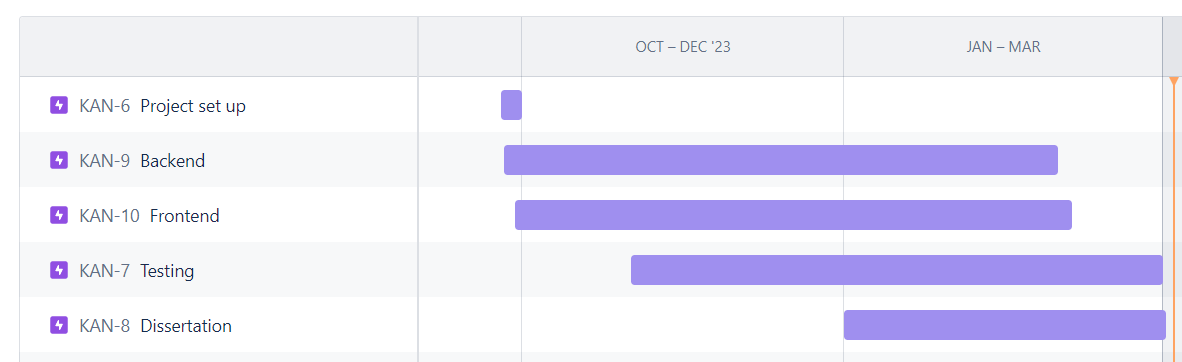
\includegraphics[width=0.7\textwidth]{images/jira.PNG}
    \caption{Jira timeline}
    \label{fig:jira-timeline}
\end{figure}

\section{Objectives Evaluation}
ConnectSphere's overall goal was to be a social media platform that allows users to have an engaging experience with other users and be able to connect in a meaningful way. The project aimed to provide features such as posts, search, chats, messages and comments to enhance user interaction. Creating a secure user authentication to increase application security. These were some of the objectives of the project. The time constraints of the project made it very difficult to develop the application to achieve the objectives. Valuable experiences and skills were gained with the comprehensive development of MERN throughout the entire project. Learned to successfully apply the best practices for MERN stack technologies. The project included the conception, design, and development of a full-fledged web application. This project honed the developer's project management skills and provided valuable experience.


\subsection{Enhance User Engagement}
Implementation of features such as posts, likes, dislikes, videos, images and user interactions have been successfully added. Users can create posts, interact with them through likes and comments, and share images or videos. Dynamic content support for updating and deleting user-generated posts has been successfully implemented, allowing users to manage their content dynamically. This goal was achieved, allowing users to have control over their posts. Users can follow and unfollow other users on ConnectSphere, and a recommendation system has been implemented to suggest users to follow. This goal was achieved by facilitating social connection and enchaining user engagement through recommendation follows. A search has been implemented that allows users to search for another user by username.  Searches are responsive and provide relevant user suggestions. This goal has been successfully achieved, allowing users to efficiently discover and connect with other users. 

User profiles have been created to display key user data and follower counts, providing users with comprehensive user information about their user profiles and social interaction. Successful implementation of key features contribute to the strength of the application. Other features such as a notifications, live chat and messaging have been added to the platform, helping users to stay connected. Time constraints may have impacted the depth of some features or functionality, potentially limiting their scalability. Figure 5.2 depicts the platform's message page.

\begin{figure}[h!]
    \centering
    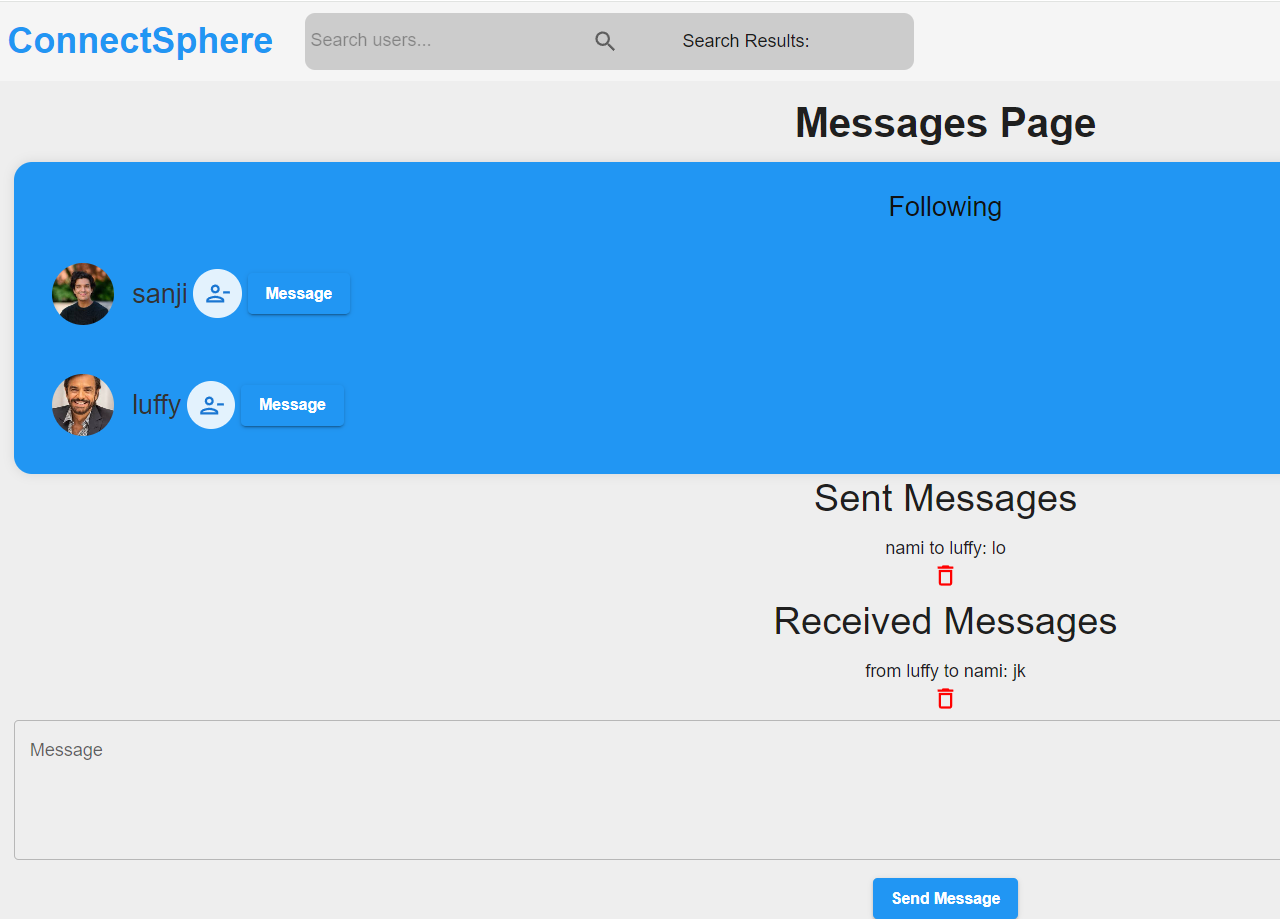
\includegraphics[width=0.7\textwidth]{images/message.PNG}
    \caption{Message Page}
    \label{fig:message-page}
\end{figure}

\subsection{Secure User Authentication}
Secure user authentication is an important part of the application, especially for the sensitive user data or to facilitate interactions between users. In this project, secure authentication was achieved by implementing of token-based authentication. A token-based user authentication system has been implemented for user login and registration. This ensures secure access to accounts and protecting sensitive information. Secure user authentication has been successfully achieved, providing users with a secure and reliable authentication mechanism. User passwords are securely hashed and protected from unauthorized access even in the event of a data breach. Only authenticated users with a valid token can access protected resources using token-based authentication. The web application is resilient against common security vulnerabilities, increasing the overall stability of the authentication system. Using
standard security practices such as JWT for authentication and bcrypt for password hashing ensures user authentication best practices are followed.

Maintaining and updating the authentication system to address evolving security threats and compliance requirements can be complex and resource intensive. The secure user authentication implemented in the project provides a solid foundation for protecting user accounts and sensitive data. Best practices of authentication and continuous system monitoring and updating allow the application to maintain a high level of security and user trust. Although the project includes key features such as authentication, social interaction, and content discovery, it may lack some advanced features found in mature social media platforms. Future iterations of the project may expand functionality. 

\section{Project Testing}
Testing is an essential part of ensuring the reliability and security of ConnectSphere. In this project, Postman was the primary method for testing the backend, covering the multiple scenarios to evaluate the overall performance and functionality of the web application. Other testing methods included unit testing, user acceptance testing, and integration testing. Each API endpoint, including user authentication, post creation, user search and profile management, has been tested by Postman. Various HTTP methods such as GET, PATCH, POST and DELETE were used to communicate with the different endpoints and validate their behavior. Authentication endpoints such as login and registration have been tested to ensure that users can authenticate and securely access protected resources. The design of the API endpoints had to match the expected results. The check included valid inputs, invalid inputs and unauthorized access attempts. Data validation and error handling were part of the process. The input validation and error handling mechanism has been tested to ensure that the application correctly detects and handles invalid input and error conditions. Tests were performed to simulate scenarios such as missing parameters, incorrect queries, and server errors. Some load tests were performed to evaluate the performance of the web application at different levels of concurrent user activity. This was important because scalability issues can arise as the user base grows, requiring optimization to handle increased traffic and load. 

Postman helped identify and resolve bugs, and inconsistencies in the backend API, improving the overall robustness and reliability of the social media platform. Extensive testing of authentication endpoints ensured that user authentication and authorization mechanisms were functioning properly, protecting user accounts and data. All the features such as messaging, login, post creation, search, profile management and interactions have been covered in the testing approach to ensure complete coverage of the application features. Authentication endpoints testing validated the implementation of secure token-based authentication and protected against security vulnerabilities, ensuring compliance with best practices. Integration testing was performed to verify interactions between different components of the web application to ensure seamless functionality across the entire platform. Overall, testing with Postman played a critical role in validating the functionality, security, and performance of the project's backend API.

\section{Database}
Database schemas are designed to efficiently store and retrieve user-related data such as user information, authentication credentials, post, and messages. Collections are organized to support the relationship between users and their posts, followers and other entities, enabling efficient querying and data retrieval. MongoDB enabled fast and efficient queries and provided quick access to user data, posts, and messages. MongoDB scalability and sharding capabilities have provided the foundation for scaling the database as the web application's user base grows. MongoDB flexible schema design allowed for easy adaption to changing application requirements and user needs. integrating MongoDB as the project database provided a solid foundation for storing, managing and retrieving project content. Its flexibility and scalability features met the project requirements and supported the development of a reliable and responsive web application.

\section{Socket.Io}
Socket.Io enabled real-time, two-way communication between the client and server, enabling instant updates and interaction within the application. Users can join chat rooms, send messages, and receive updates without having to manually refresh the entire site. Real-time features like live chats and notifications helps increase user engagement by enabling seamless communication. Users can chat with each other in real time, fostering a sense of communication and enabling meaningful interaction on the platform.
Socket.IO architecture and web sockets support ensures scalable communication with concurrent users. Socket.IO plays a key role in enabling real-time interactions and improving user engagement within the application. Robust features allow users to communicate and stay informed in real time, creating a vibrant user community. A chat room where two users can send messages to each other is shown in Figure 5.3. Figure 5.4 shows the notification page with users liking post notify.

\begin{figure}[h!]
    \centering
    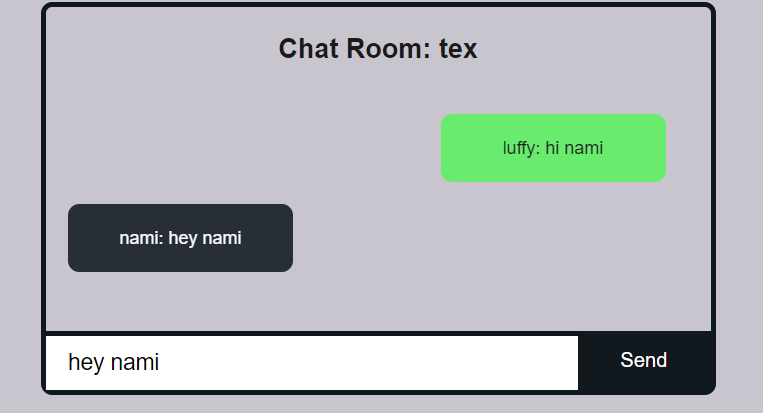
\includegraphics[width=0.7\textwidth]{images/chatroom.PNG}
    \caption{Chat Page}
    \label{fig:chat-rooms}
\end{figure}

\begin{figure}[h!]
    \centering
    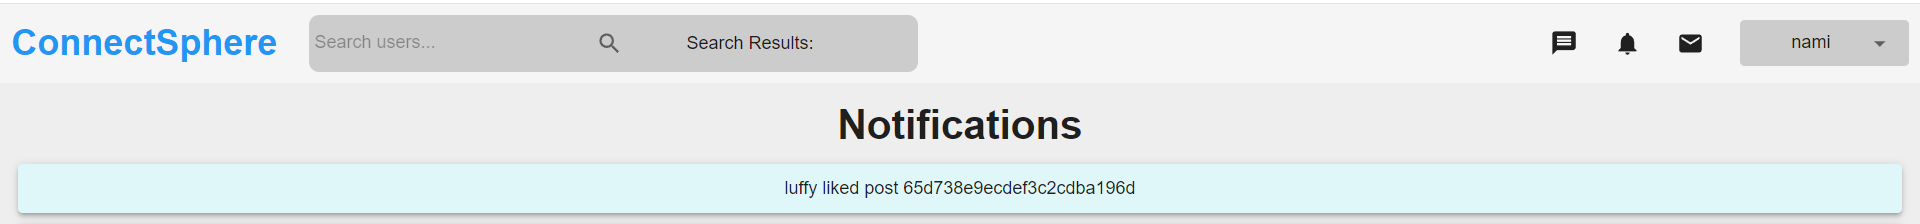
\includegraphics[width=0.7\textwidth]{images/notify.PNG}
    \caption{Notification Page}
    \label{fig:like-notify}
\end{figure}

\section{Frontend and Backend}
\subsection{Frontend}
Frontend components is characterized by its responsiveness and ensuring a seamless experience across different devices. Responsive design principles associated with Material-UI, contribute to a visually appealing and user-friendly interface. State management techniques such as Redux are used effectively to manage application state. Socket.IO integration enables real-time communication and enhance user engagement with features like live chats and notifications. Token-based authentication mechanisms ensure secure user registration and login processes, protect user data and improve overall system security. Authentication follows best practices. The navigation and routing mechanisms created by React Router enables seamless navigation between different views and pages within the web application. Users can easily navigate between features such as user profiles, chat rooms, message inbox page, home page and notification page, improving usability and accessibility. 

Testing strategies such as unit tests and integration tests that help identify code issues and bugs. Frontend development took a long time compared to the backend development. Many HTTP request issues that took some time to solve. Solving these problems took effort to fix.

\subsection{Backend}
The backend is well structured and follows best practices, promoting modularity and scalability. Separation of concerns and use of middleware capabilities contribute to a robust and extensible backend architecture. Token-based authentication mechanisms, implemented using libraries such as JWT, provide secure user authentication and authorization for users. Authentication endpoints comply with MERN standards and include features such as password hashing to improve security. Integration with MongoDB facilitates efficient data storage and retrieval. Data models and schemas are well defined, support CRUD operations, and ensure data consistency and integrity. Integration with Socket.IO enables real time communication between the server and client, facilitating features such as live chats and notifications. The backend worked as expected and was able to perform the task required by the social media platform.  

\subsection{Deployment}
Deploying the web application on Render marks a significant success in the project life-cycle, demonstrating the ability to move from local development to a production environment. Despite the challenges encountered during the deployment process, such as resolving URL issues in frontend HTTP requests. The local-host URLs in the frontend had to be replaced with the new URL provided by Render. For deployment to work, the bcrypt library also had to be removed. Instead, the bcrpty.js library was used to resolve the deployment issues. Deploying the application on Render has several advantages. Render provides scalability allowing ConnectSphere to remain responsive and available during periods of increased activity. Hosting the application on Render improves its reliability and availability. Overall, the successful deployment to Render reflects the ability to overcome challenges and adapt to new environments. This success highlights the project's ability to be used in the real world and creates a solid foundation for development and growth.